\documentclass[../240513_msquare_shor.tex]{subfiles}

\begin{document}

\subsection*{}

\begin{frame}{Theoretical Computer Science}
    \begin{center}
        \begin{minipage}{.8\linewidth}
        Theoretical computer science is a subfield of computer science and \fbox{mathematics} that
        focuses on the abstract and mathematical foundations of computation, such as the theory of
        computation, formal language theory, the lambda calculus and type theory.
        \end{minipage}
    \end{center}
    \hfill \textit{Theoretical computer science}, Wikipedia.
\end{frame}

\begin{frame}<1-| handout:0>{Theoretical Computer Science}
    \begin{figure}
        \centering
        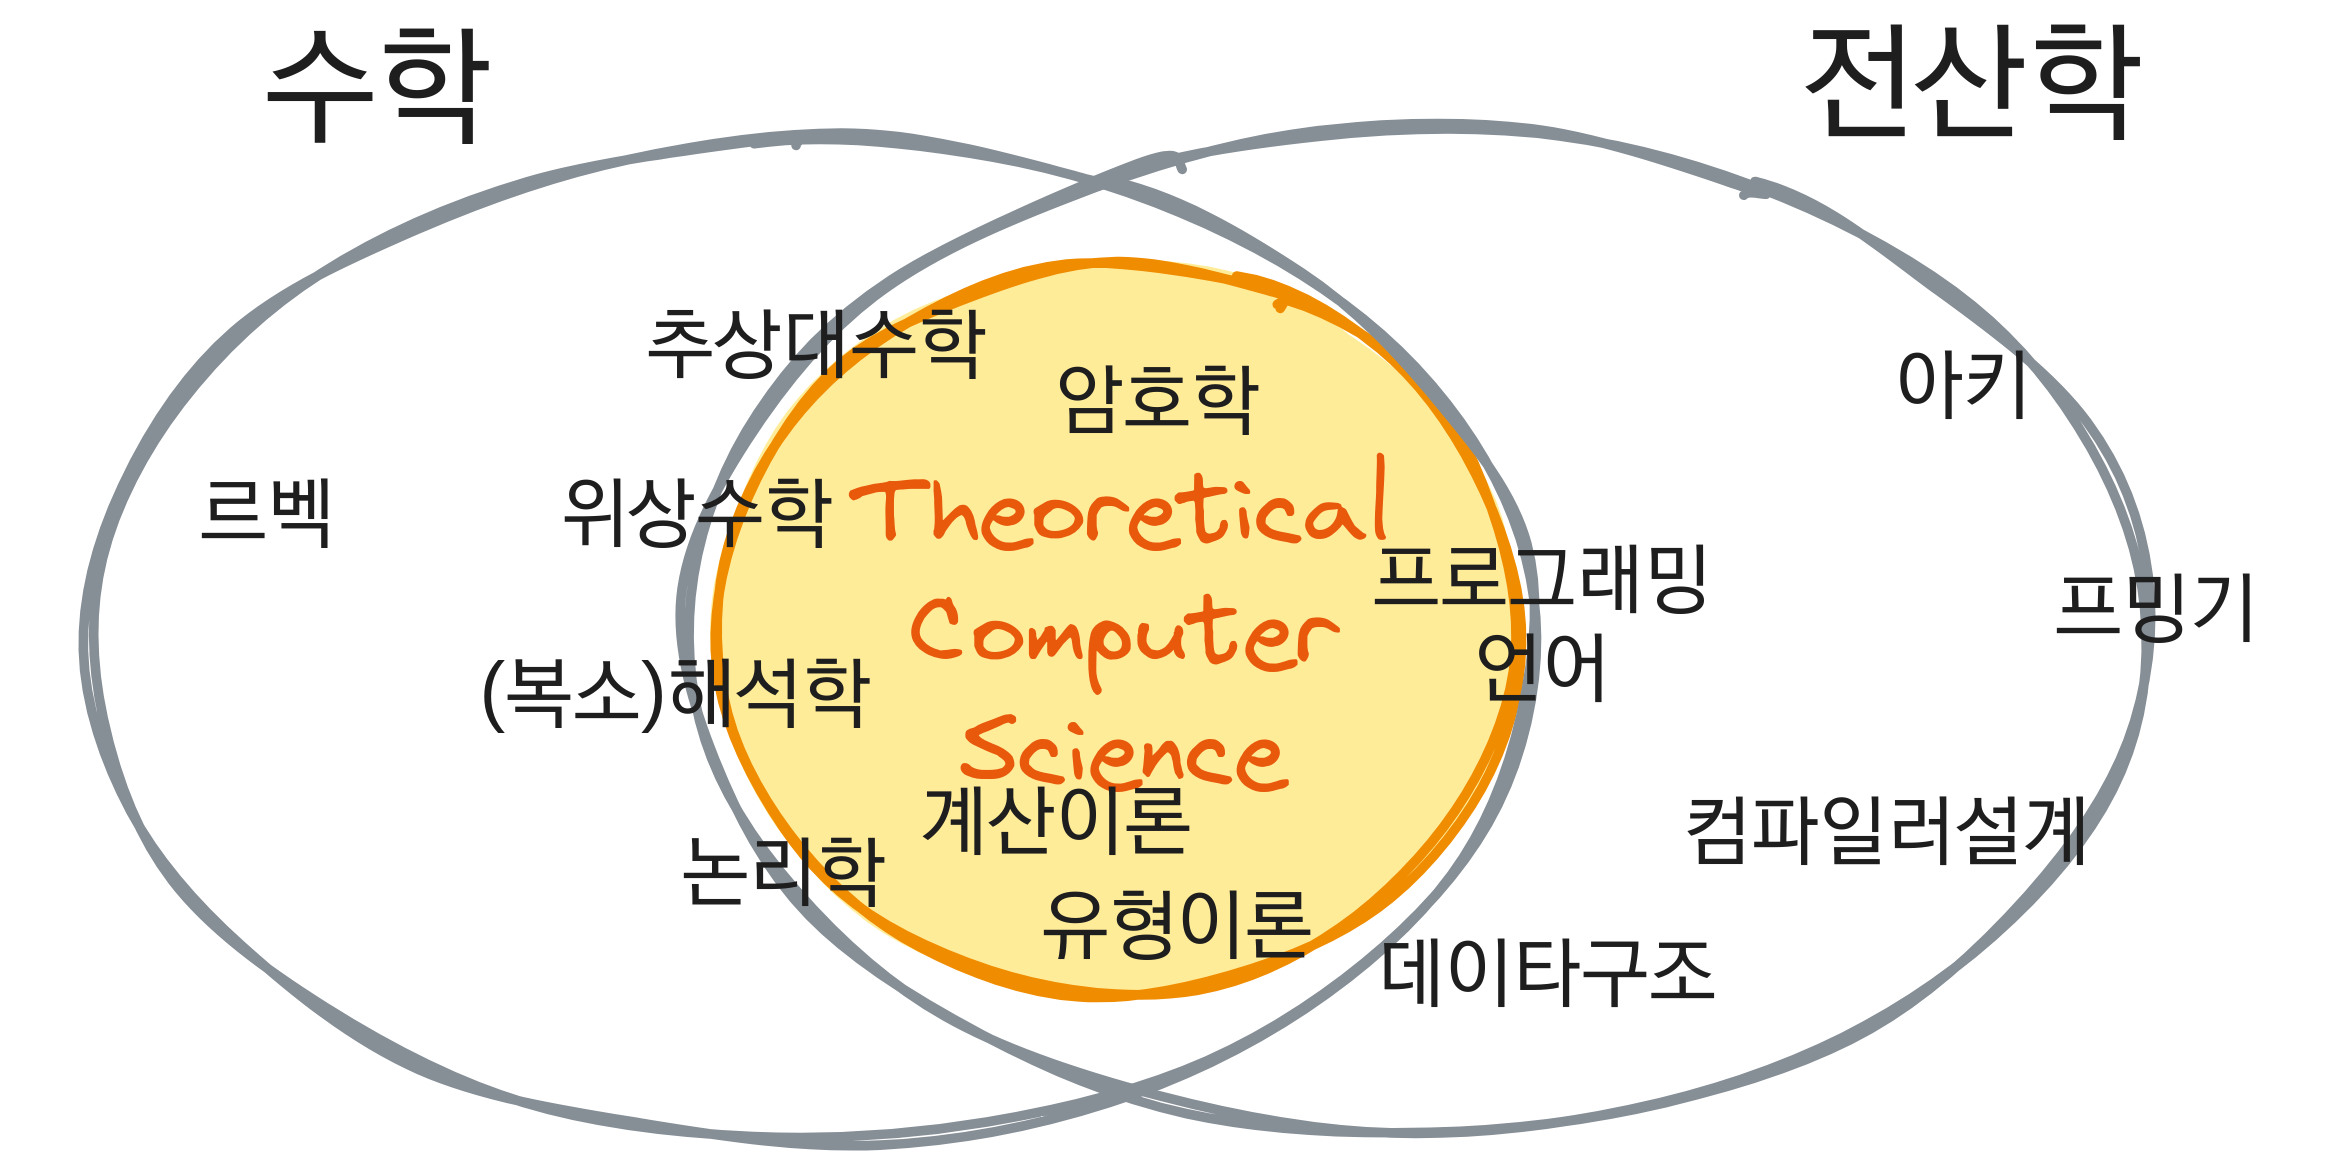
\includegraphics[width=\textwidth]{images/theoretical_computer_science1.png}
    \end{figure}
\end{frame}

\begin{frame}{Theoretical Computer Science}
    \begin{figure}
        \centering
        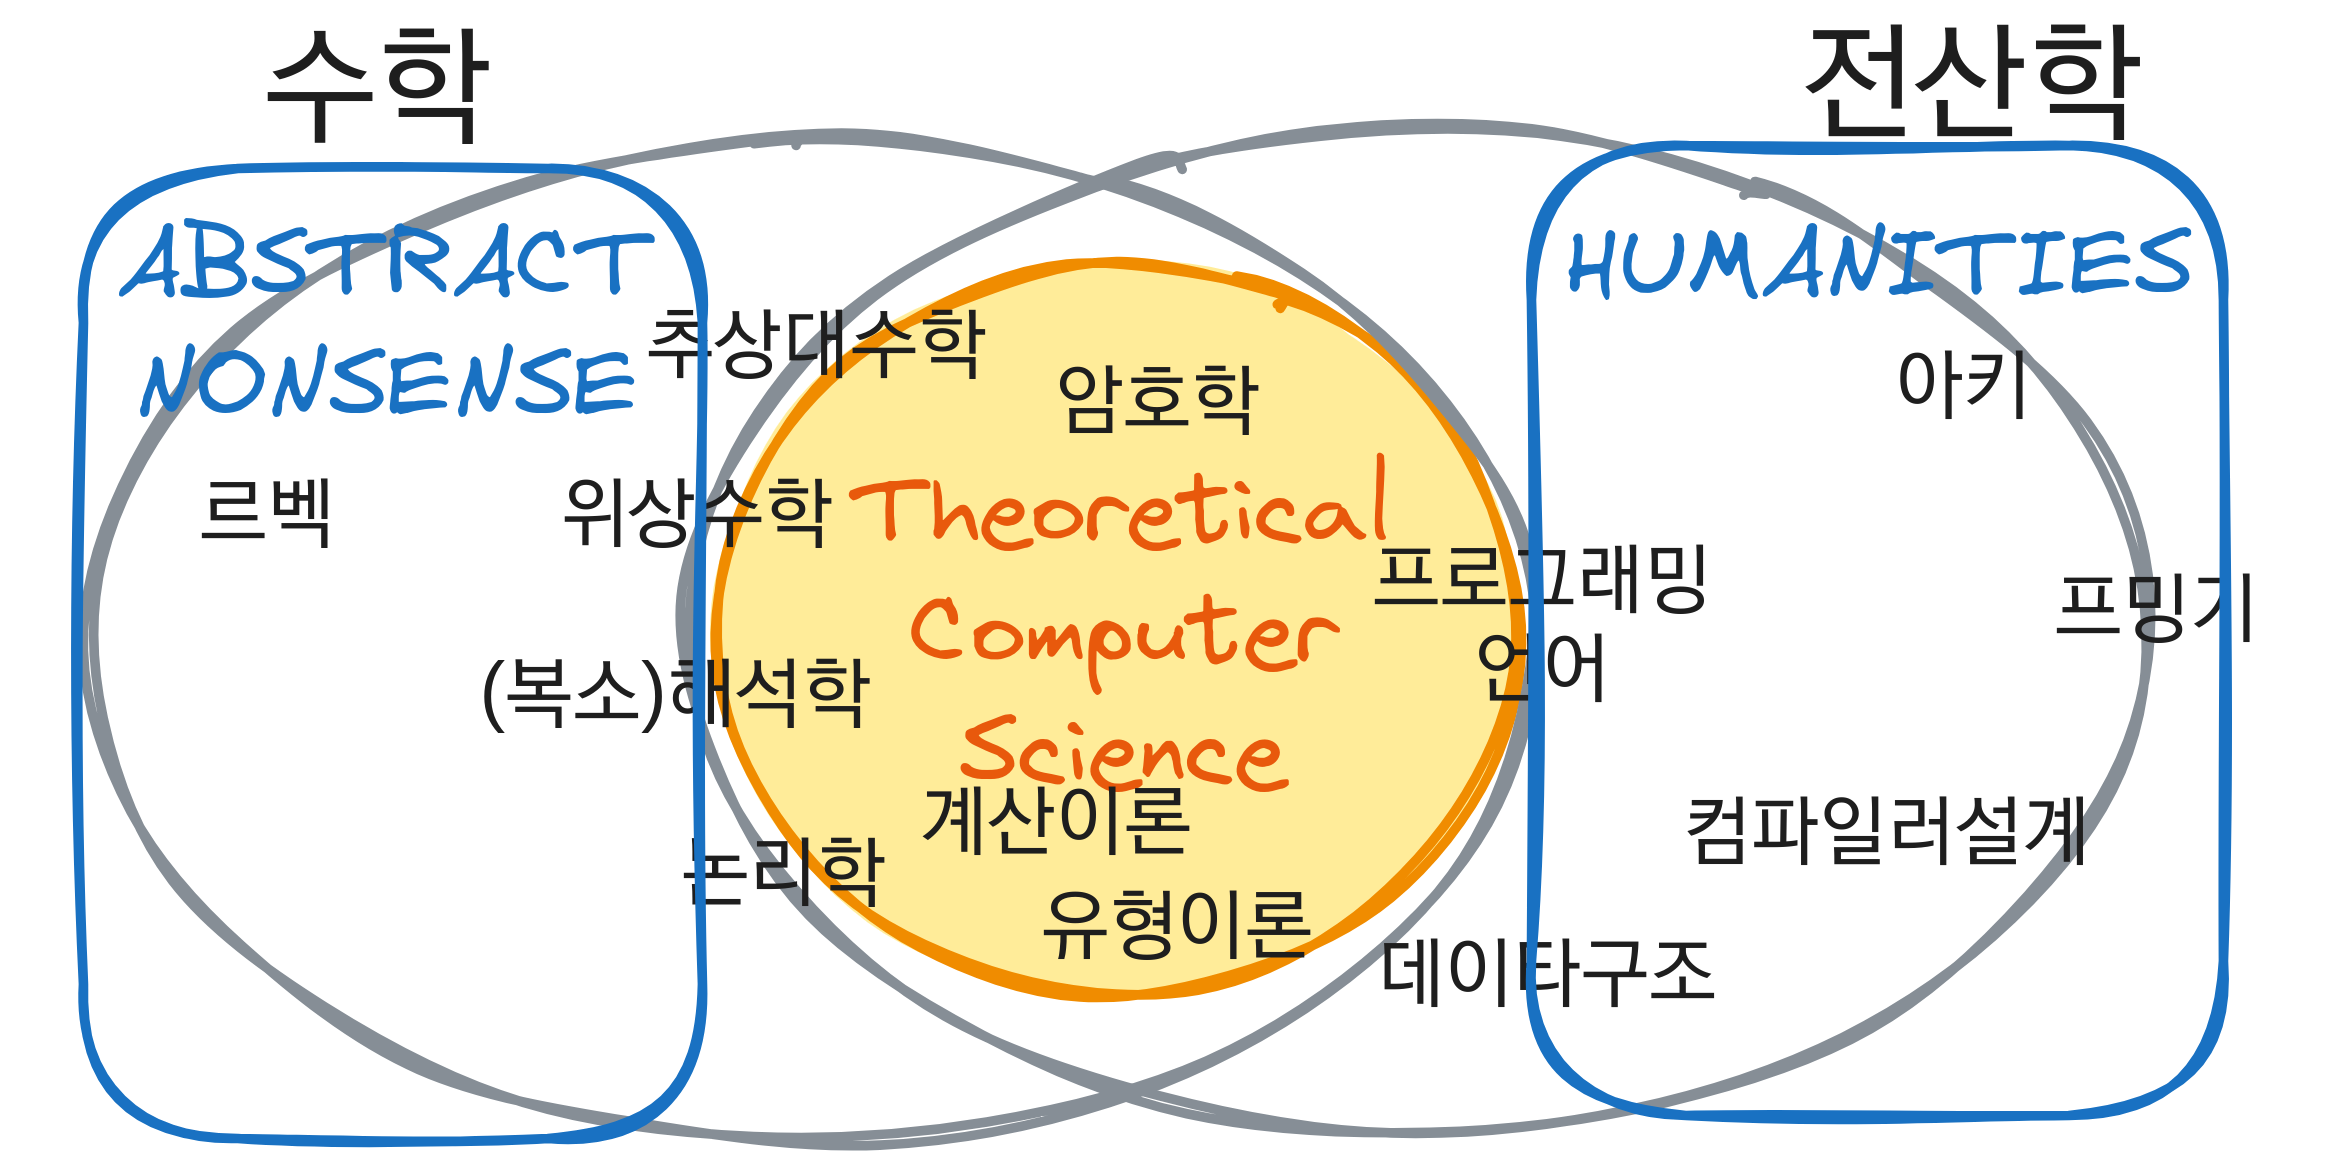
\includegraphics[width=\textwidth]{images/theoretical_computer_science2.png}
    \end{figure}
\end{frame}

\begin{frame}{Two Different Perspectives}
    \begin{exampleblock}{}
        \begin{center}
            \(\gcd(a,b)\)를 바라보는 두 가지 시각
        \end{center}
    \end{exampleblock}
    \pause
    \begin{columns}
        \column{.5\textwidth}
        \begin{figure}
            \centering
            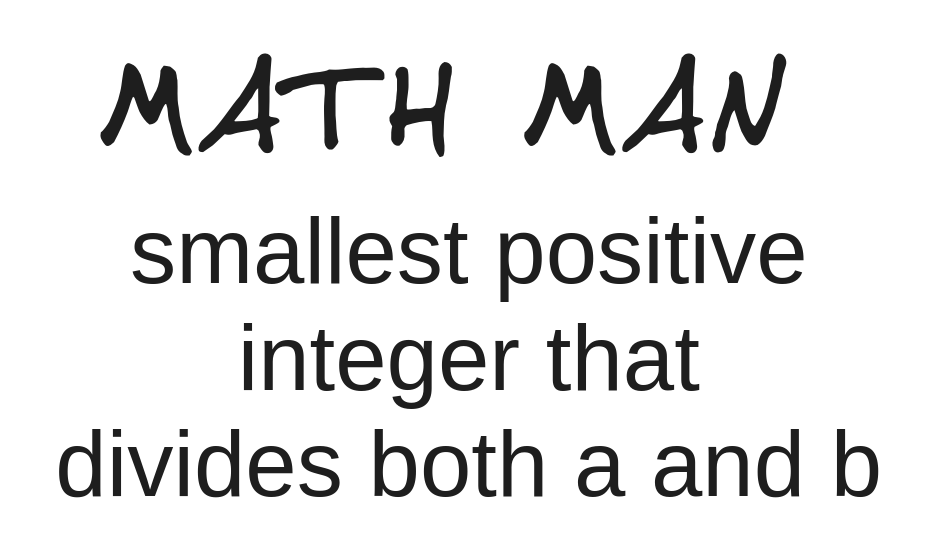
\includegraphics[width=\textwidth]{images/gcd_math.png}
        \end{figure}
        \centering
        존재성, 유일성, 정의에서 오는 여러 정리...
        \column{.5\textwidth}
        \pause
        \begin{figure}
            \centering
            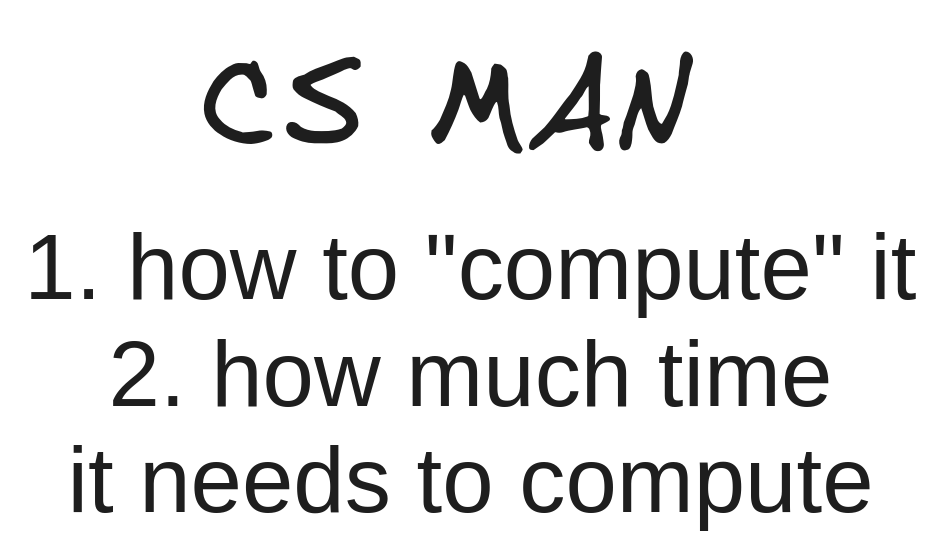
\includegraphics[width=\textwidth]{images/gcd_cs.png}
        \end{figure}
        \centering
        효율적으로 "계산"할 수 없으면 다른 유용한 것을 계산하는 데 사용할 수 없음
    \end{columns}
    \pause
    \vfill
    \centering
    오늘 세미나를 CS Man의 시각에서 보면 더 재미있을 것임!
\end{frame}

\subsection{Example}

\begin{frame}{RSA Cryptosystem}
    \begin{exampleblock}{Euler's Theorem}
        If \(\gcd(x, N) = 1\), then \(x^{\phi(N)} \equiv 1 \pmod{N}\).
    \end{exampleblock}
    \pause
    \begin{block}{RSA Cryptosystem}
        \begin{enumerate}
            \ii
            천지원이 최푸른하늘한테 메시지 \(m \in \NN\)을 보내고 싶어 함.
            \ii
            최푸른하늘은 큰 소수 \(p, q\)를 골라서 \(N = pq\)를 계산함.
            \ii
            최푸른하늘은 또 \(\phi(N) = (p-1)(q-1)\)과 서로소인 적당한 \(e\)를 골라서
            \(ed \equiv 1 \pmod{\phi(N)}\)인 \(d\)를 계산함
            \ii
            최푸른하늘은 모두에게 \(N\)과 \(e\)를 공개함.
            \ii
            천지원은 \(c = x^e \text{ mod }N\)을 계산해서 모두에게 공개함
            \ii
            최푸른하늘은 \(m = c^d \text{ mod }N\)을 계산할 수 있음
            \ii
            \alert{다른 사람은 \(d\)을 계산할 수 없기 때문에 최푸른하늘만 \(m\)을 해독할 수 있음}
        \end{enumerate}
    \end{block}
\end{frame}

\begin{frame}{RSA Cryptosystem: Calculation}
    \begin{alertblock}{정수에 대한 Time Complexity}
        어떤 문제에 대한 input이 정수 \(N\)일 때는 input의 크기를 \(\log N\)으로 봄.
        (\(N\)을 표현하는 데 \(\log N\) 개의 글자가 필요해서)
        예를 들어 시간 복잡도가 \(O(N)\)이면 poly-time이 아니라 \(O(2^{\log N})\), 즉 exponential time임.
    \end{alertblock}
    \pause
    \begin{block}{Modular Exponentiation}
        \(x^e \text{ mod } N\)을 어떻게 계산할까? Time complexity는?
    \end{block}
\end{frame}

\end{document}
